\chapter{BEL2ABM: agent-based simulation of static models in Biological Expression Language}
\label{ch:bel2abm}

\section*{Preface}

While previous chapters have improved the ability of \ac{BEL} to model multi-modal and multi-scale aspects of complex disease while integrating content from both unstructured text and structured sources, it has been limited by its inability to express the temporal dimension of the underlying biology.
Even further, the time scales corresponding to molecular and clinically measurable process differ by several orders of magnitude.
While others have focused on modeling timescales on the clinical level, the following publication presents a workflow (BEL2ABM) for converting knowledge graphs in \ac{BEL} into dynamic, executable, agent-based models.

\vspace*{\fill}

Reprinted with permission from "Gündel, M., Hoyt, C.T., \& Hofmann-Apitius, M. (2018). BEL2ABM: Agent-based simulation of static models in Biological Expression Language. \textit{Bioinformatics}, 34(13), 2316–2318.".
Copyright © Gündel, M., \textit{et al.}, 2018.

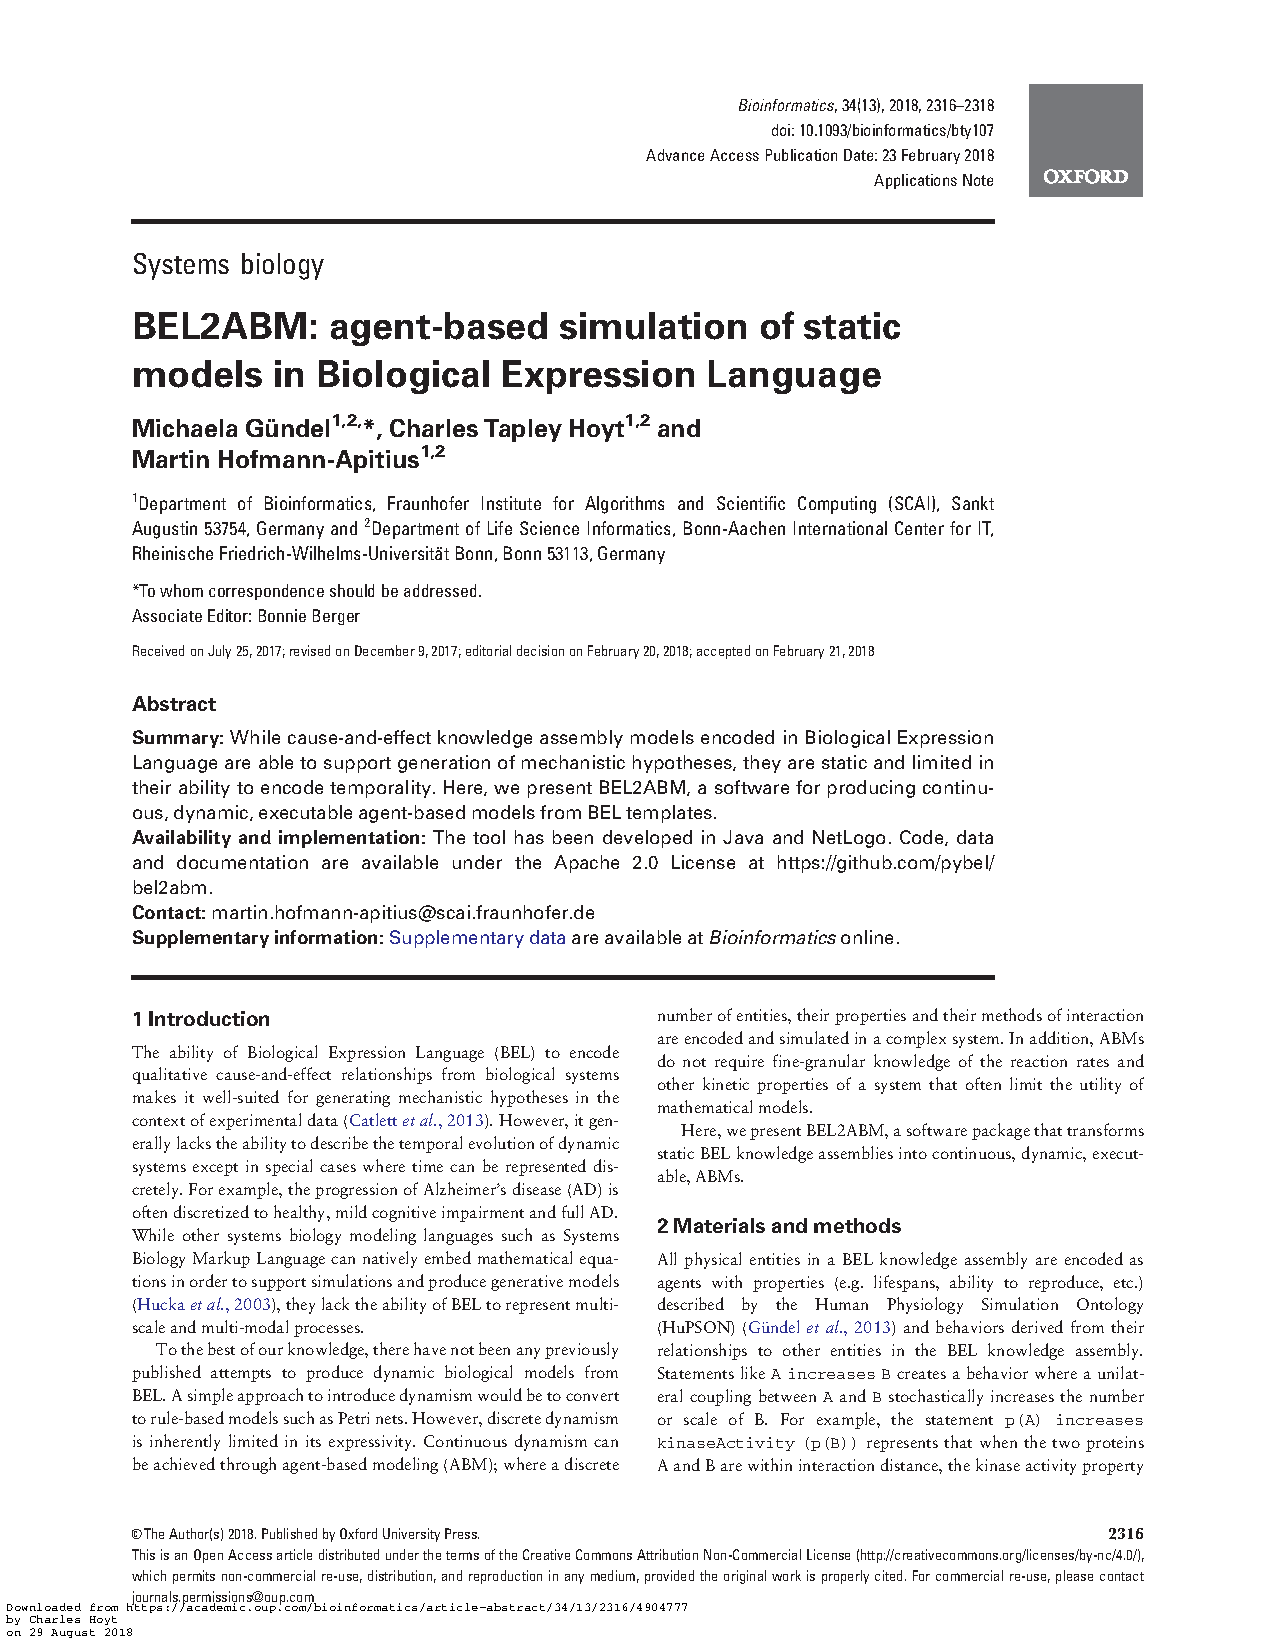
\includepdf[pages={-}]{articles/bel2abm.pdf}

\section*{Postface}

A proof of concept was presented that successfully reproduced the results of a past analysis based on an ordinary differential equation model describing the amyloid cascade from Schmidt \textit{et al.}~\cite{Schmidt2012} using a \ac{BEL} model of the amyloid cascade as an input to BEL2ABM\@.
While BEL2ABM currently only supports a small subset of the events that can be expressed in \ac{BEL}, it represents a first step towards the ability to automatically generate dynamic models from static knowledge.
Combine with the ability to automatically generate and maintain knowledge graphs containing the highest quality content from structured sources as presented in Chapter~\ref{ch:bio2bel} and new relevant content from unstructured sources as presented in Chapter~\ref{ch:recuration}, this framework is one option to overcome previously described challenges faced by both more simple and more powerful modeling techniques.
